\documentclass[12pt]{article}
\usepackage{hyperref}
\usepackage{ifpdf}
\usepackage{natbib}


\ifpdf 
   \pdfcompresslevel=9
   \pdfoutput=1
                                                                                      
      
                       
   \usepackage[pdftex]{graphicx}
   \usepackage[pdftex]{geometry}
   \usepackage[pdftex]{color}
   \usepackage{hyperref}
   \hypersetup{
     pdftitle={A Stochastic Model of a Local Deer Population and
       Associated Bond Fund},
     pdfsubject={ODE},
     pdfauthor={Kelly Black, Candace Liu, Lindong Zhou, Elizabeth Sweeney},
     pdfkeywords={Logistic Equation, Stochastic Differential
       Equations,Bond Funds},
     anchorcolor = {red},
     colorlinks = {true},
     %pdfpagemode={FullScreen}
   }
\else
   \usepackage{epsfig}
   \usepackage{color}
\fi


\makeatletter
\renewcommand{\section}{\@startsection
  {section}
  {1}
  {0em}
  {\baselineskip}
  {-1em}
  {\normalfont\normalsize\bfseries}}

\renewcommand{\subsection}{\@startsection
  {subsection}
  {2}
  {0em}
  {\baselineskip}
  {-1em}
  {\normalfont\normalsize\bfseries}}

\renewcommand{\subsubsection}{\@startsection
  {subsubsection}
  {2}
  {0em}
  {\baselineskip}
  {-2em}
  {\normalfont\normalsize\itshape}}

\renewcommand{\thesection}{\@arabic\c@section}
\renewcommand{\thesubsection}{\thesection.\@arabic\c@subsection}
\renewcommand{\thesubsubsection}{\thesubsection .\@arabic\c@subsubsection}

\makeatother

\setcounter{secnumdepth}{0}


\begin{document}

\begin{center}
  \textbf{A Stochastic Model of a Local Deer Population and Associated Bond Fund} \\
  Kelly Black\footnote{Clarkson University, Department of Mathematics
    and Computer Science, \texttt{kjblack@gmail.com}},
    Candace Liu\footnote{Clarkson University, Department of Mathematics
      and Computer Science, \texttt{liucg@clarkson.edu}},
    Lindong Zhou\footnote{Middlebury College, Department of Mathematics, 
      \texttt{lindongz@middlebury.edu}}, 
    Elizabeth Sweeney\footnote{The College of New Jersey, Department of Mathematics, 
      \texttt{sweenee1@tcnj.edu}}
\end{center}


\begin{abstract}
\end{abstract}


Keywords: Logistic Equation, Stochastic Differential Equations,Bond Funds




\section{Introduction}

This is the introduction. This is why this is important.

This is what other people did.

This paper is organized as follows. First we address a topic relevant
to the issues raised by Schwabe, and we examine the sensitivity of the
total harvest rate with the associated the parameters associated with
the harvest. Second we Examine the model for the larger system
including both the deer population and the bond fund used to back
potential liabilities associated with claims arising from automobile
collisions with deer. Third, we examine the simulations of the deer
population and discuss the range of unknown parameters associated with
the numerical explorations. Fourth we examine the results of the
simulations followed by the conclusions that can be drawn from the
simulations.

%%% Local Variables: 
%%% mode: latex
%%% TeX-master: "deerFundModeling"
%%% End: 



\section{Harvesting And Sensitivity}

An issue that arises in the study by Schwabe \textit{et al} is the
sensitivity of the total rate of harvest with the associated
parameters. Here we examine the expected total rate of harvest at
steady state as a function of the parameters that arise in a logistic
equation with a proportional harvest term. We find that there is a
maximum harvest that occurs in the middle of the possible range of
values for the parameter.

Need an overview of the section.



%%% Local Variables: 
%%% mode: latex
%%% TeX-master: "deerFundModeling"
%%% End: 



\section{Model}

\begin{frame}
    \frametitle{Stochastics}
	\begin{itemize}
		\item Brownian Motion (Random Walks) - $W(t)$
		\item Properties
	\begin{enumerate}[i]
		\item $W(t)$ is continuous
		\item $W(t)$ is no where differentiable
		\item If $t_{1}<t_{2}<t_{3}<t_{4}$, \\
			$W(t_{1}), W(t_{2})-W(t_{1}),  W(t_{3})-W(t_{4})$ are independent random variables
		\item If $0 \le s\le t$ then $W(t)-W(s) \sim N(0, t-s)$
	\end{enumerate}
		\item Gaussian White ``Noise" - $dW$
	\end{itemize}
%%%%%%%%%% Brownian Motion, Gaussian White Noise
\end{frame}



\begin{frame}
    \frametitle{Models}
	\begin{eqnarray}
		dx &=& \tilde{r} x \left( 1- \frac{x}{\tilde{f}}\right) dt +\alpha x \, dW \\
		dm &=& ( \rho m - \beta x + P) dt - \gamma x \, dW
	\end{eqnarray}
	\begin{itemize}
		\item Known Parameters - $\tilde{r}$, $\tilde{f}$, $\rho$, $\beta$
		\item Unknown Parameters - $\alpha$, $\gamma$, $P$
	\end{itemize}
\end{frame}




\section{Numerics}

\begin{frame}
   \frametitle{Approximation}
%%%%%%%%%Include figure
\vspace*{-3em}
	\begin{eqnarray*}
		dX &=& f(X) \, dt + g(X) \, dW \\
	\end{eqnarray*}
\vspace*{-3em}
	\begin{center}
		$X_{j} =$ approximation of $X(t_{j})$ \\ [20pt]
	\includegraphics[height=4cm]{approximation}
	\end{center}

\end{frame}



\begin{frame}
    \frametitle{Methods of Approximations}
	Euler-Maruyama Method - $O(\Delta t^{1})$
	\begin{eqnarray*}
		X_{j} &=& X_{j-1} + f(X_{j-1})\triangle t+ g(X_{j-1})(W(\tau_{j})-W(\tau_{j-1})) \\
		 j &=& 1,2,... ,L \\
	\end{eqnarray*}
	Milstein Method - $O(\Delta t^{1.5})$
	\begin{eqnarray*}
		X_{j} &=& X_{j-1} + \triangle tf(X_{j-1}) + g(X_{j-1})(W(\tau_{j})-W(\tau_{j-1})) 	\nonumber\\ 
		&& + \frac{1}{2} g(X_{j-1})g'(X_{j-1})((W(\tau_{j})-W(\tau_{j-1}))^{2}-\triangle t)\\
		 j &=& 1,2,... ,L \\
	\end{eqnarray*}
\end{frame}


\begin{frame}
    \frametitle{Benchmark}
	\framesubtitle{Paths}
\hspace*{-2cm}
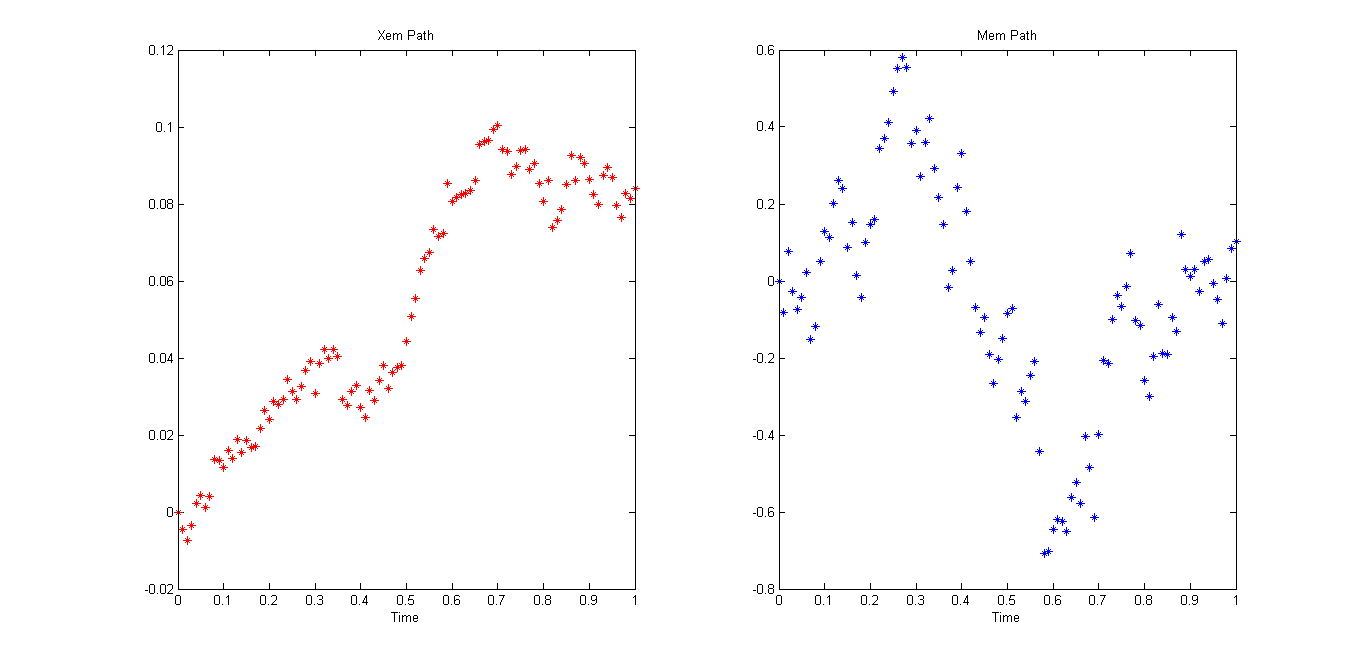
\includegraphics[height=7cm]{testpaths} 
\end{frame}


\begin{frame}
    \frametitle{Benchmark}
	\framesubtitle{Histogram}
\hspace*{-5mm}
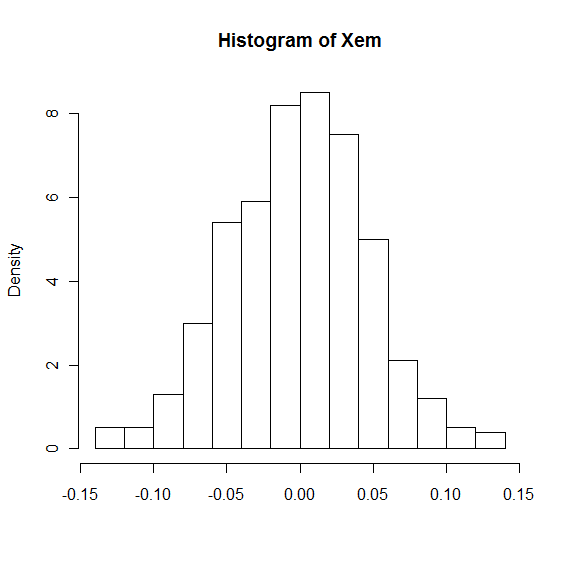
\includegraphics[height=6cm]{testhistX}
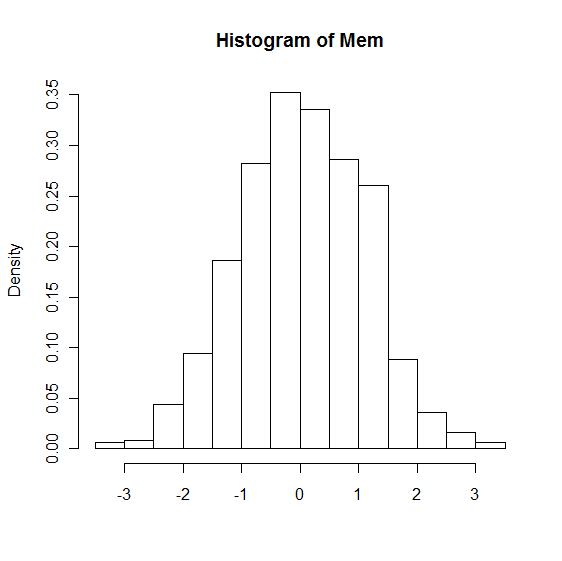
\includegraphics[height=6cm]{testhistM}
\end{frame}


\begin{frame}
    \frametitle{Benchmark}
	\framesubtitle{95\% Confidence Interval}
\begin{center}
	$\bar{x} \pm t_{(\alpha /2, df=n-1)} \frac{s}{\sqrt{n}}$ \\ 
\vspace{5mm}
\begin{tabular}{r c l c r c l}
	$E[X]$ &=& 0 && $E[M]$ &=& 0 \\
	$Var[X]$ &=& 0.0025  && $Var[M]$ &=& 1 
\end{tabular}
\end{center}
\begin{itemize}
	\item $\bar{X}$ (-0.0104, 0.00826)
	\item $\bar{M}$ (-0.172, 0.252)
\end{itemize}
\end{frame}


\begin{frame}
    \frametitle{Parameter Space}
\hspace*{-2cm}
%%%%%%%%%% Include 3D plot of parameter space
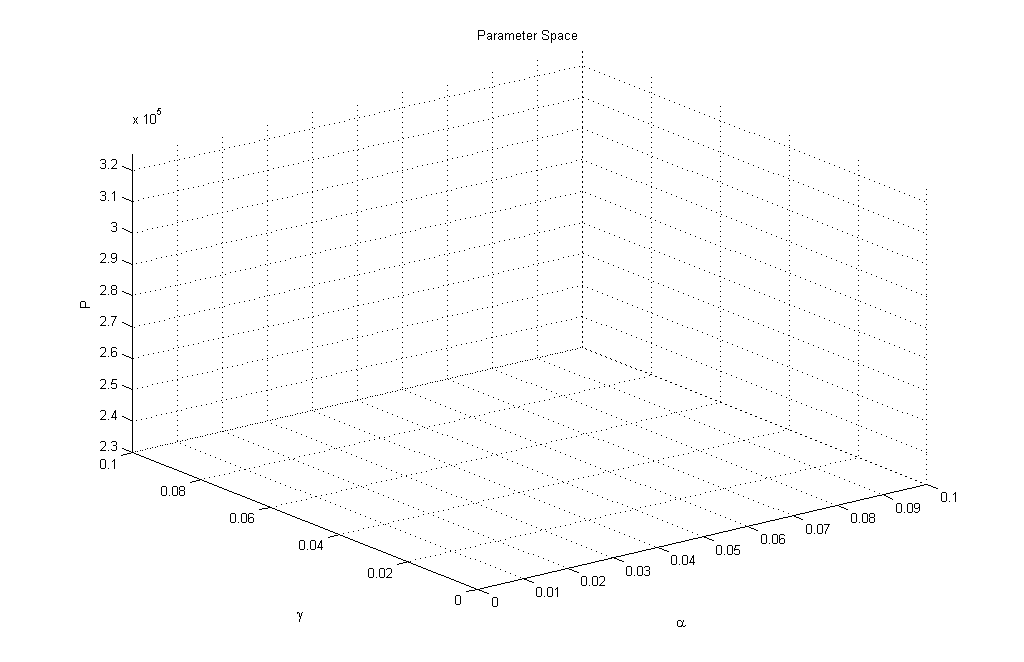
\includegraphics[height=7cm]{parameterspace}
\end{frame}







\section{Monte Carlo Simulations}

Need an overview and outline for this section.

Include an overview of the parameter space.

Include an overview of the numerical approximation.

Include the details of the implementation. Cite the github repository
\cite{deerActuaryRepo}.  Cite our use of R \cite{R}.

%%% Local Variables: 
%%% mode: latex
%%% TeX-master: "deerFundModeling"
%%% End: 






\section{Results}

\begin{frame}
    \frametitle{Results - Example for One Run}
\vspace*{-1cm}
\begin{eqnarray*}
\begin{array}{r c l r c l r c l}
	\alpha &=& .05, & \gamma &=& .05, & P &=& 230000
\end{array}
\end{eqnarray*}
\hspace*{-2cm}
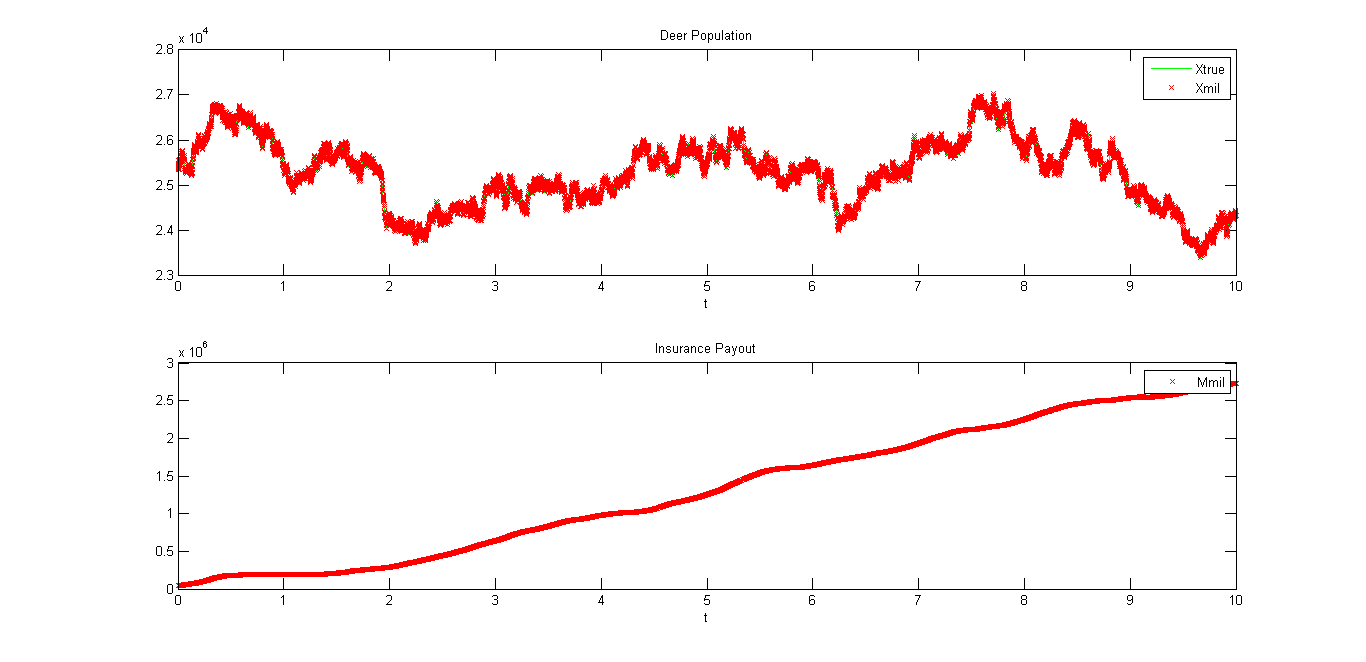
\includegraphics[height=7cm]{deerins}
\end{frame}


\begin{frame}
    \frametitle{Results - X vs. alpha }
	\framesubtitle{500 iterations}
\hspace*{-5mm}
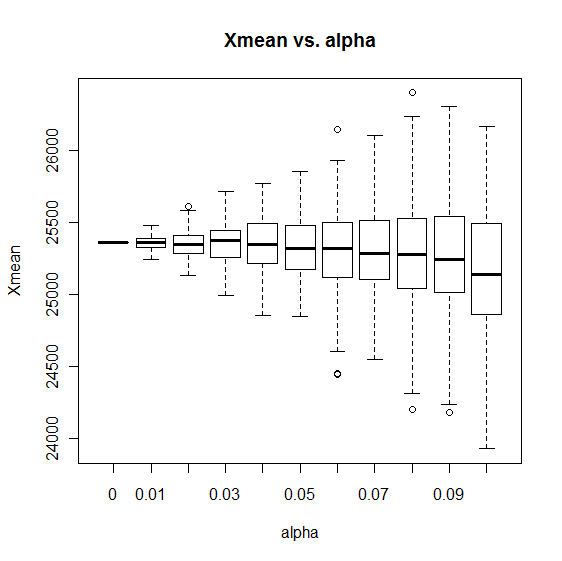
\includegraphics[height=6cm]{boxplot500_xmean_alpha}
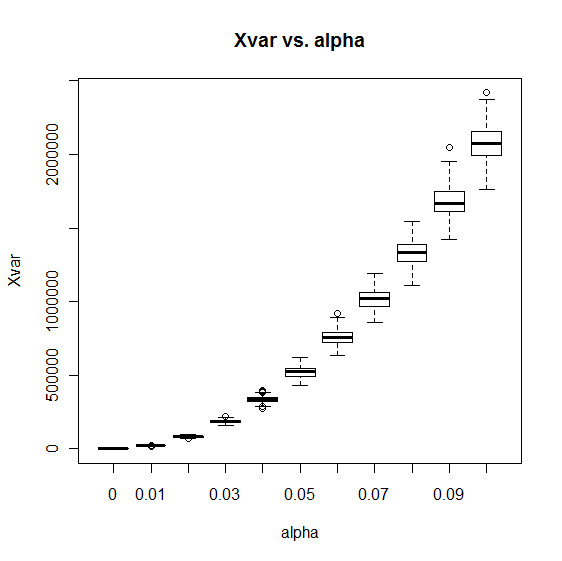
\includegraphics[height=6cm]{boxplot500_xvar_alpha}
\end{frame}

\begin{frame}
    \frametitle{Results - X vs. alpha }
	\framesubtitle{1000 iterations}
\hspace*{-5mm}
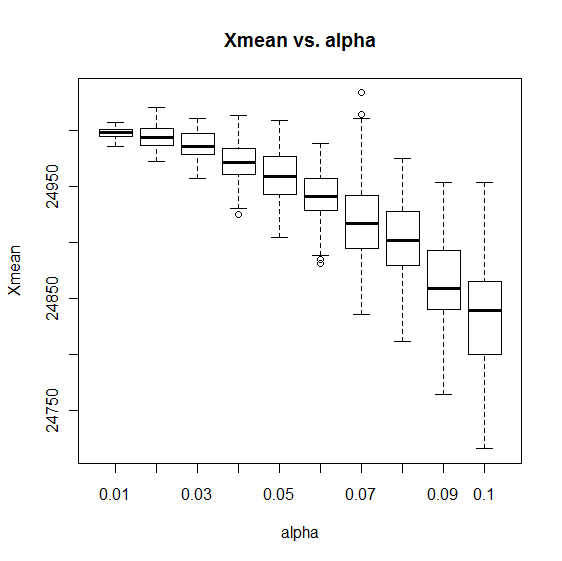
\includegraphics[height=6cm]{boxplot1000_xmean_alpha}
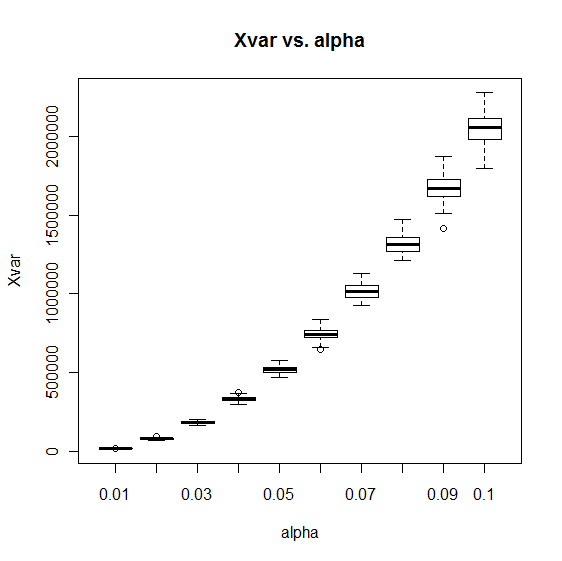
\includegraphics[height=6cm]{boxplot1000_xvar_alpha}
\end{frame}

\begin{frame}
    \frametitle{Results - Histogram}
	\framesubtitle{1000 iterations}
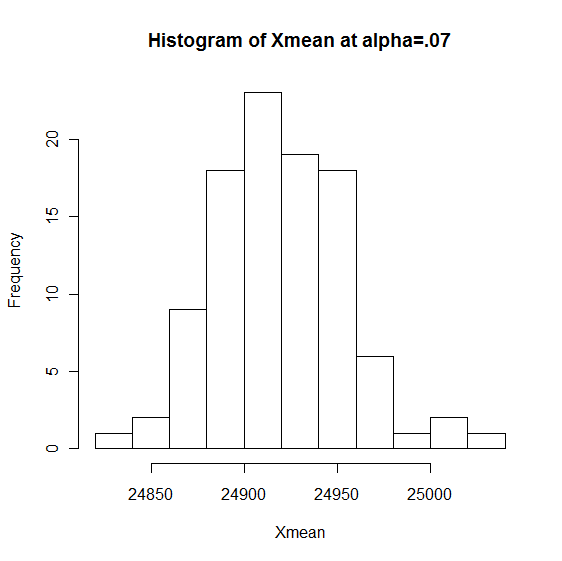
\includegraphics[height=6cm]{hist1000_xmean_alpha07}
\end{frame}



\begin{frame}
    \frametitle{Results - M vs. alpha }
	\framesubtitle{500 iterations}
\hspace*{-5mm}
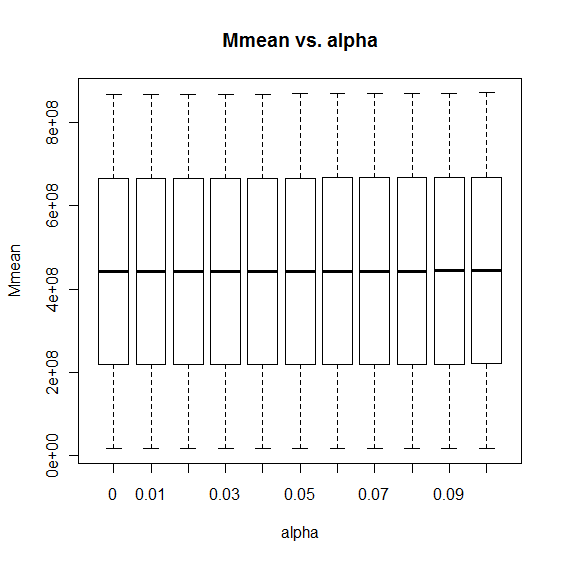
\includegraphics[height=6cm]{boxplot500_mmean_alpha}
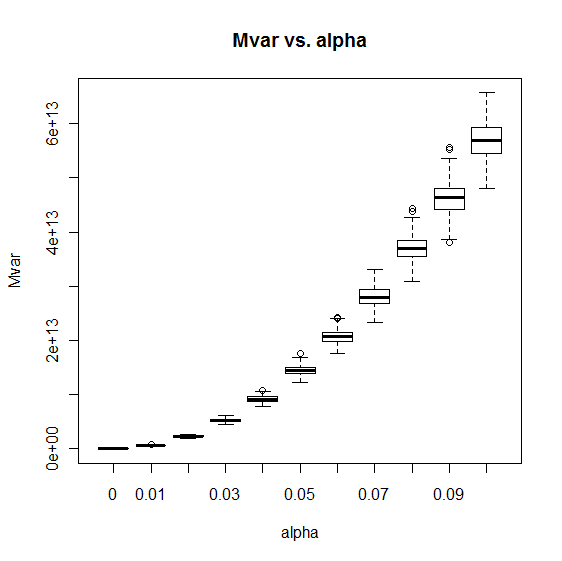
\includegraphics[height=6cm]{boxplot500_mvar_alpha}
\end{frame}

\begin{frame}
    \frametitle{Results - M vs. alpha }
	\framesubtitle{1000 iterations}
\hspace*{-5mm}
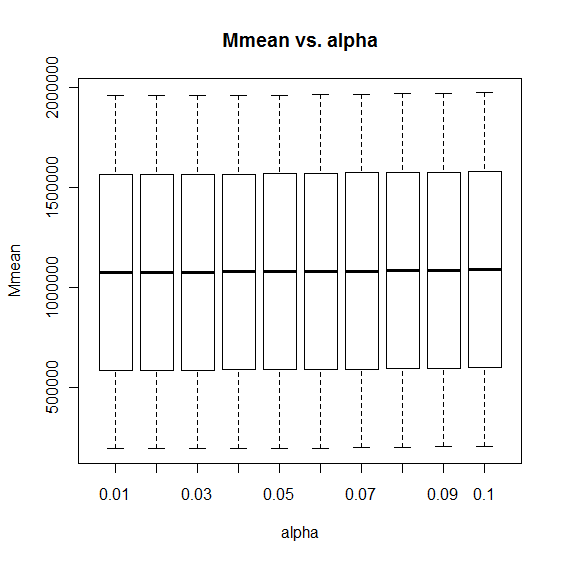
\includegraphics[height=6cm]{boxplot1000_mmean_alpha}
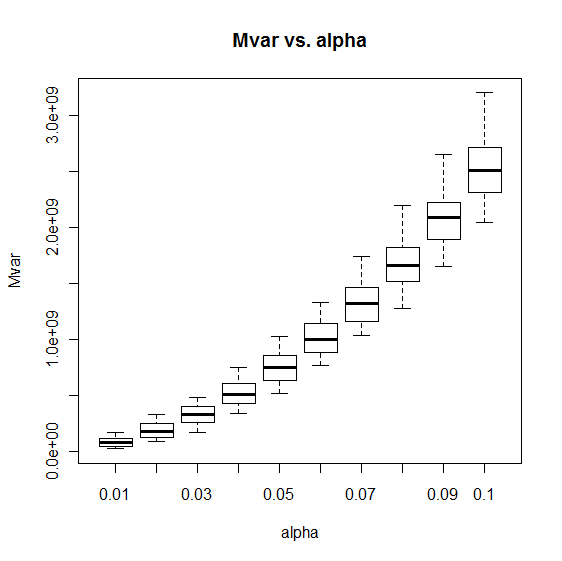
\includegraphics[height=6cm]{boxplot1000_mvar_alpha}
\end{frame}



\begin{frame}
    \frametitle{Results - M vs. gamma }
	\framesubtitle{500 iterations}
\hspace*{-5mm}
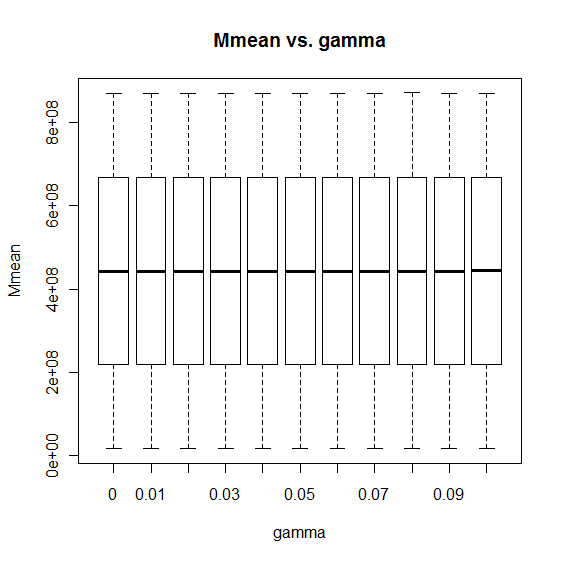
\includegraphics[height=6cm]{boxplot500_mmean_gamma}
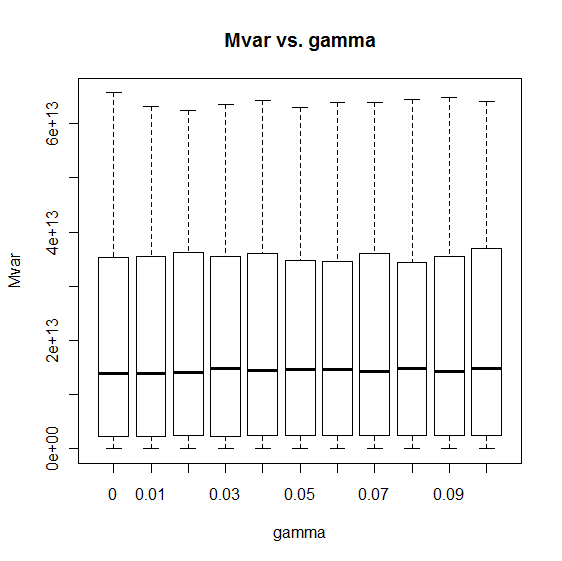
\includegraphics[height=6cm]{boxplot500_mvar_gamma}
\end{frame}

\begin{frame}
    \frametitle{Results - M vs. gamma }
	\framesubtitle{1000 iterations}
\hspace*{-5mm}
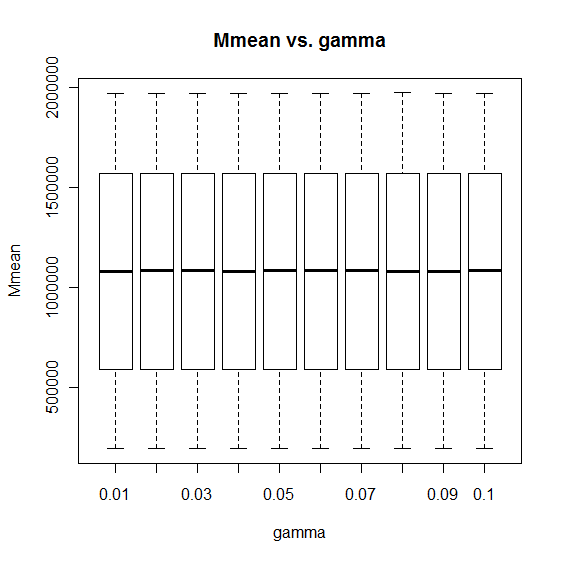
\includegraphics[height=6cm]{boxplot1000_mmean_gamma}
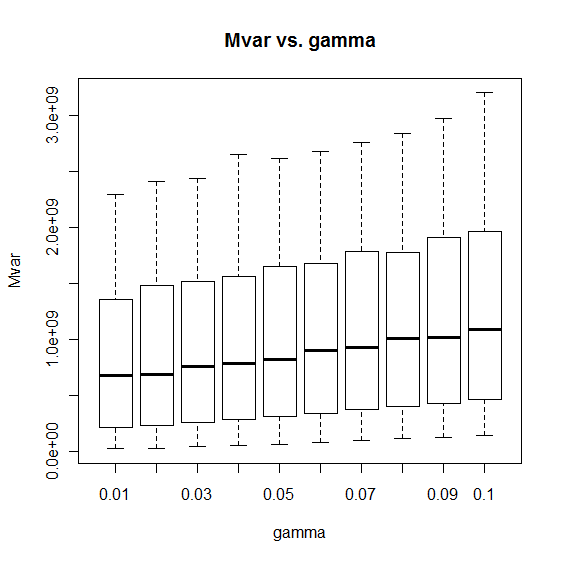
\includegraphics[height=6cm]{boxplot1000_mvar_gamma}
\end{frame}





\begin{frame}
    \frametitle{Results - M vs. P }
	\framesubtitle{500 iterations}
\hspace*{-5mm}
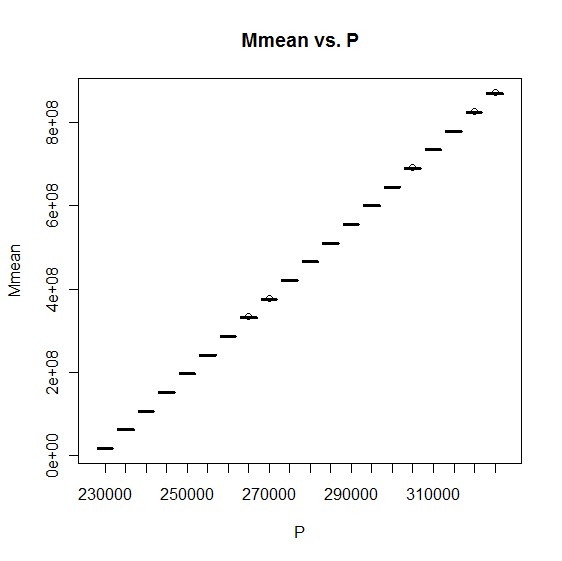
\includegraphics[height=6cm]{boxplot500_mmean_P}
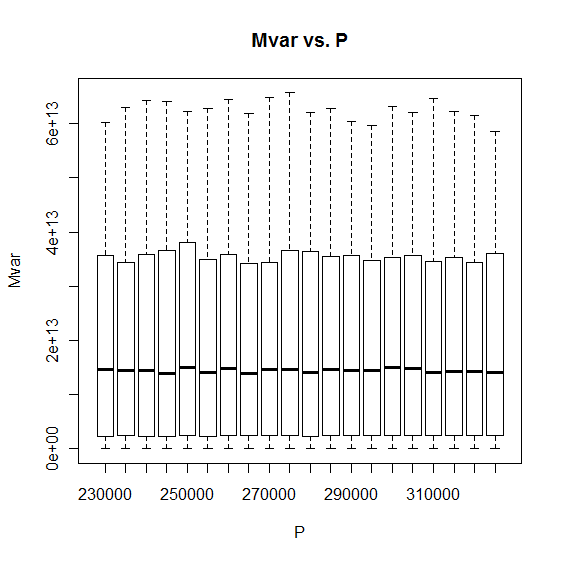
\includegraphics[height=6cm]{boxplot500_mvar_P}
\end{frame}


\begin{frame}
    \frametitle{Results - M vs. P }
	\framesubtitle{1000 iterations}
\hspace*{-5mm}
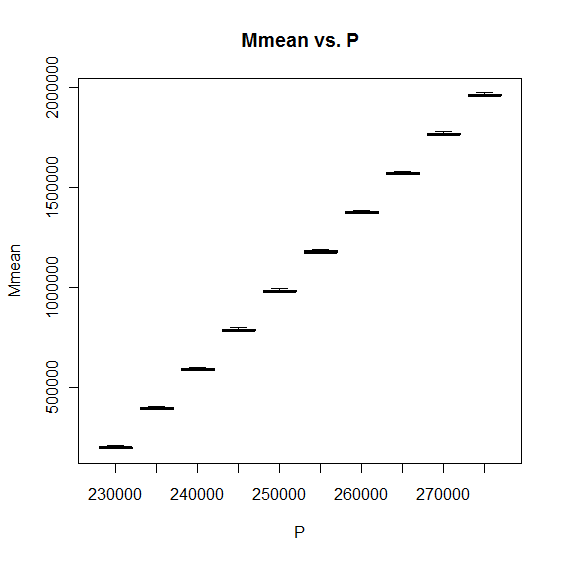
\includegraphics[height=6cm]{boxplot1000_mmean_P}
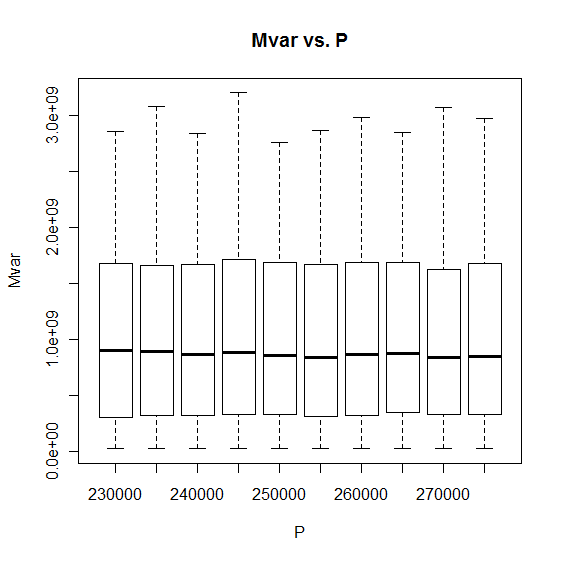
\includegraphics[height=6cm]{boxplot1000_mvar_P}
\end{frame}


\begin{frame}
    \frametitle{Video Simulations}

	\url{ https://www.youtube.com/watch?v=g-rqa3chaq8}

	\url{https://www.youtube.com/watch?v=RcQfMBF8-Og}

\end{frame}



\section{Conclusions}

\begin{frame}
    \frametitle{Conclusion}
\begin{itemize}
	\item Stochastic Model of Deer-Collisions and Insurance Bond Funds 
	\item Consistent with basic benchmarks
	\item System most sensitive to $\alpha$
	\item Linear relationship between $M$ and $P$
	\item Initial $M$ may be too big
	\item Multivariate sensitivity should be examined
\end{itemize}
\end{frame}







\section{Conclusions}

Discuss our conclusions here.

\section{Acknowledgements}

We wish to thank Dr. Joel Foisy, Chair of the Department of
Mathematics at the State University of New York at Potsdam as well as
the National Science Foundation (NSF1262737). Their support made
possible by the Research Experience for Undergraduates program enabled
us to explore this topic and provided an invaluable experience for all
participants.


%%% Local Variables: 
%%% mode: latex
%%% TeX-master: "deerFundModeling"
%%% End: 


\bibliographystyle{chicago}
\bibliography{sde}



\end{document}

%%% Local Variables: 
%%% mode: latex
%%% TeX-master: t
%%% End: 
